% Options for packages loaded elsewhere
\PassOptionsToPackage{unicode}{hyperref}
\PassOptionsToPackage{hyphens}{url}
%
\documentclass[
]{article}
\title{Project 2 Notebook}
\author{}
\date{\vspace{-2.5em}}

\usepackage{amsmath,amssymb}
\usepackage{lmodern}
\usepackage{iftex}
\ifPDFTeX
  \usepackage[T1]{fontenc}
  \usepackage[utf8]{inputenc}
  \usepackage{textcomp} % provide euro and other symbols
\else % if luatex or xetex
  \usepackage{unicode-math}
  \defaultfontfeatures{Scale=MatchLowercase}
  \defaultfontfeatures[\rmfamily]{Ligatures=TeX,Scale=1}
\fi
% Use upquote if available, for straight quotes in verbatim environments
\IfFileExists{upquote.sty}{\usepackage{upquote}}{}
\IfFileExists{microtype.sty}{% use microtype if available
  \usepackage[]{microtype}
  \UseMicrotypeSet[protrusion]{basicmath} % disable protrusion for tt fonts
}{}
\makeatletter
\@ifundefined{KOMAClassName}{% if non-KOMA class
  \IfFileExists{parskip.sty}{%
    \usepackage{parskip}
  }{% else
    \setlength{\parindent}{0pt}
    \setlength{\parskip}{6pt plus 2pt minus 1pt}}
}{% if KOMA class
  \KOMAoptions{parskip=half}}
\makeatother
\usepackage{xcolor}
\IfFileExists{xurl.sty}{\usepackage{xurl}}{} % add URL line breaks if available
\IfFileExists{bookmark.sty}{\usepackage{bookmark}}{\usepackage{hyperref}}
\hypersetup{
  pdftitle={Project 2 Notebook},
  hidelinks,
  pdfcreator={LaTeX via pandoc}}
\urlstyle{same} % disable monospaced font for URLs
\usepackage[margin=1in]{geometry}
\usepackage{color}
\usepackage{fancyvrb}
\newcommand{\VerbBar}{|}
\newcommand{\VERB}{\Verb[commandchars=\\\{\}]}
\DefineVerbatimEnvironment{Highlighting}{Verbatim}{commandchars=\\\{\}}
% Add ',fontsize=\small' for more characters per line
\usepackage{framed}
\definecolor{shadecolor}{RGB}{248,248,248}
\newenvironment{Shaded}{\begin{snugshade}}{\end{snugshade}}
\newcommand{\AlertTok}[1]{\textcolor[rgb]{0.94,0.16,0.16}{#1}}
\newcommand{\AnnotationTok}[1]{\textcolor[rgb]{0.56,0.35,0.01}{\textbf{\textit{#1}}}}
\newcommand{\AttributeTok}[1]{\textcolor[rgb]{0.77,0.63,0.00}{#1}}
\newcommand{\BaseNTok}[1]{\textcolor[rgb]{0.00,0.00,0.81}{#1}}
\newcommand{\BuiltInTok}[1]{#1}
\newcommand{\CharTok}[1]{\textcolor[rgb]{0.31,0.60,0.02}{#1}}
\newcommand{\CommentTok}[1]{\textcolor[rgb]{0.56,0.35,0.01}{\textit{#1}}}
\newcommand{\CommentVarTok}[1]{\textcolor[rgb]{0.56,0.35,0.01}{\textbf{\textit{#1}}}}
\newcommand{\ConstantTok}[1]{\textcolor[rgb]{0.00,0.00,0.00}{#1}}
\newcommand{\ControlFlowTok}[1]{\textcolor[rgb]{0.13,0.29,0.53}{\textbf{#1}}}
\newcommand{\DataTypeTok}[1]{\textcolor[rgb]{0.13,0.29,0.53}{#1}}
\newcommand{\DecValTok}[1]{\textcolor[rgb]{0.00,0.00,0.81}{#1}}
\newcommand{\DocumentationTok}[1]{\textcolor[rgb]{0.56,0.35,0.01}{\textbf{\textit{#1}}}}
\newcommand{\ErrorTok}[1]{\textcolor[rgb]{0.64,0.00,0.00}{\textbf{#1}}}
\newcommand{\ExtensionTok}[1]{#1}
\newcommand{\FloatTok}[1]{\textcolor[rgb]{0.00,0.00,0.81}{#1}}
\newcommand{\FunctionTok}[1]{\textcolor[rgb]{0.00,0.00,0.00}{#1}}
\newcommand{\ImportTok}[1]{#1}
\newcommand{\InformationTok}[1]{\textcolor[rgb]{0.56,0.35,0.01}{\textbf{\textit{#1}}}}
\newcommand{\KeywordTok}[1]{\textcolor[rgb]{0.13,0.29,0.53}{\textbf{#1}}}
\newcommand{\NormalTok}[1]{#1}
\newcommand{\OperatorTok}[1]{\textcolor[rgb]{0.81,0.36,0.00}{\textbf{#1}}}
\newcommand{\OtherTok}[1]{\textcolor[rgb]{0.56,0.35,0.01}{#1}}
\newcommand{\PreprocessorTok}[1]{\textcolor[rgb]{0.56,0.35,0.01}{\textit{#1}}}
\newcommand{\RegionMarkerTok}[1]{#1}
\newcommand{\SpecialCharTok}[1]{\textcolor[rgb]{0.00,0.00,0.00}{#1}}
\newcommand{\SpecialStringTok}[1]{\textcolor[rgb]{0.31,0.60,0.02}{#1}}
\newcommand{\StringTok}[1]{\textcolor[rgb]{0.31,0.60,0.02}{#1}}
\newcommand{\VariableTok}[1]{\textcolor[rgb]{0.00,0.00,0.00}{#1}}
\newcommand{\VerbatimStringTok}[1]{\textcolor[rgb]{0.31,0.60,0.02}{#1}}
\newcommand{\WarningTok}[1]{\textcolor[rgb]{0.56,0.35,0.01}{\textbf{\textit{#1}}}}
\usepackage{graphicx}
\makeatletter
\def\maxwidth{\ifdim\Gin@nat@width>\linewidth\linewidth\else\Gin@nat@width\fi}
\def\maxheight{\ifdim\Gin@nat@height>\textheight\textheight\else\Gin@nat@height\fi}
\makeatother
% Scale images if necessary, so that they will not overflow the page
% margins by default, and it is still possible to overwrite the defaults
% using explicit options in \includegraphics[width, height, ...]{}
\setkeys{Gin}{width=\maxwidth,height=\maxheight,keepaspectratio}
% Set default figure placement to htbp
\makeatletter
\def\fps@figure{htbp}
\makeatother
\setlength{\emergencystretch}{3em} % prevent overfull lines
\providecommand{\tightlist}{%
  \setlength{\itemsep}{0pt}\setlength{\parskip}{0pt}}
\setcounter{secnumdepth}{-\maxdimen} % remove section numbering
\ifLuaTeX
  \usepackage{selnolig}  % disable illegal ligatures
\fi

\begin{document}
\maketitle

\hypertarget{introduction}{%
\subsection{Introduction}\label{introduction}}

\hypertarget{scientific-question}{%
\subsubsection{Scientific Question}\label{scientific-question}}

\emph{hfi} hihiao

\begin{Shaded}
\begin{Highlighting}[]
\CommentTok{\#for reading in fasta files}
\FunctionTok{library}\NormalTok{(}\StringTok{"BiocManager"}\NormalTok{)}
\CommentTok{\#for reading in excel files}
\FunctionTok{library}\NormalTok{(}\StringTok{"readxl"}\NormalTok{)}
\CommentTok{\#forgot}
\FunctionTok{library}\NormalTok{(}\StringTok{"seqinr"}\NormalTok{)}
\CommentTok{\#for multiple sequence alignment }
\FunctionTok{library}\NormalTok{(}\StringTok{"msa"}\NormalTok{)}
\end{Highlighting}
\end{Shaded}

\begin{verbatim}
## Loading required package: Biostrings
\end{verbatim}

\begin{verbatim}
## Loading required package: BiocGenerics
\end{verbatim}

\begin{verbatim}
## 
## Attaching package: 'BiocGenerics'
\end{verbatim}

\begin{verbatim}
## The following objects are masked from 'package:stats':
## 
##     IQR, mad, sd, var, xtabs
\end{verbatim}

\begin{verbatim}
## The following objects are masked from 'package:base':
## 
##     anyDuplicated, append, as.data.frame, basename, cbind, colnames,
##     dirname, do.call, duplicated, eval, evalq, Filter, Find, get, grep,
##     grepl, intersect, is.unsorted, lapply, Map, mapply, match, mget,
##     order, paste, pmax, pmax.int, pmin, pmin.int, Position, rank,
##     rbind, Reduce, rownames, sapply, setdiff, sort, table, tapply,
##     union, unique, unsplit, which.max, which.min
\end{verbatim}

\begin{verbatim}
## Loading required package: S4Vectors
\end{verbatim}

\begin{verbatim}
## Loading required package: stats4
\end{verbatim}

\begin{verbatim}
## 
## Attaching package: 'S4Vectors'
\end{verbatim}

\begin{verbatim}
## The following objects are masked from 'package:base':
## 
##     expand.grid, I, unname
\end{verbatim}

\begin{verbatim}
## Loading required package: IRanges
\end{verbatim}

\begin{verbatim}
## Loading required package: XVector
\end{verbatim}

\begin{verbatim}
## Loading required package: GenomeInfoDb
\end{verbatim}

\begin{verbatim}
## 
## Attaching package: 'Biostrings'
\end{verbatim}

\begin{verbatim}
## The following object is masked from 'package:seqinr':
## 
##     translate
\end{verbatim}

\begin{verbatim}
## The following object is masked from 'package:base':
## 
##     strsplit
\end{verbatim}

\begin{verbatim}
## 
## Attaching package: 'msa'
\end{verbatim}

\begin{verbatim}
## The following object is masked from 'package:BiocManager':
## 
##     version
\end{verbatim}

\begin{Shaded}
\begin{Highlighting}[]
\CommentTok{\#for msa pretty print }
\FunctionTok{library}\NormalTok{(}\StringTok{"tinytex"}\NormalTok{)}
\CommentTok{\#visualization of results }
\FunctionTok{library}\NormalTok{(}\StringTok{"ggplot2"}\NormalTok{)}
\CommentTok{\#for clustering of DNA seqs }
\FunctionTok{library}\NormalTok{(}\StringTok{"DECIPHER"}\NormalTok{)}
\end{Highlighting}
\end{Shaded}

\begin{verbatim}
## Loading required package: RSQLite
\end{verbatim}

\begin{verbatim}
## Loading required package: parallel
\end{verbatim}

\begin{Shaded}
\begin{Highlighting}[]
\NormalTok{knitr}\SpecialCharTok{::}\FunctionTok{include\_graphics}\NormalTok{(}\StringTok{"dog/Basenji.jpg"}\NormalTok{)}
\end{Highlighting}
\end{Shaded}

\begin{figure}
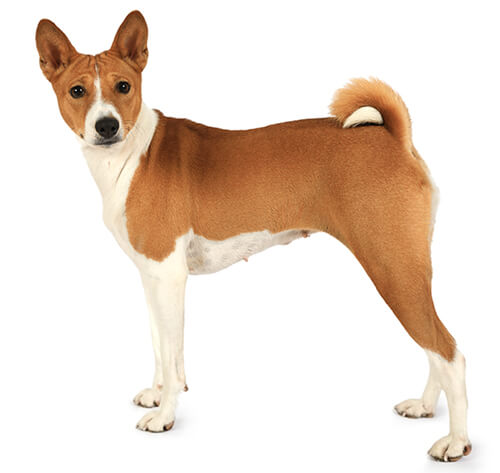
\includegraphics[width=400px]{dog/Basenji} \caption{Basenji (S)}\label{fig:unnamed-chunk-2-1}
\end{figure}

\begin{Shaded}
\begin{Highlighting}[]
\NormalTok{knitr}\SpecialCharTok{::}\FunctionTok{include\_graphics}\NormalTok{(}\StringTok{"dog/labret.jpg"}\NormalTok{)}
\end{Highlighting}
\end{Shaded}

\begin{figure}
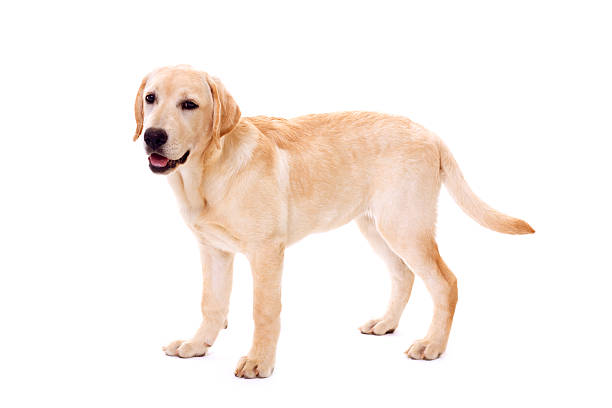
\includegraphics[width=400px]{dog/labret} \caption{Boxer (L)}\label{fig:unnamed-chunk-2-2}
\end{figure}

\begin{Shaded}
\begin{Highlighting}[]
\NormalTok{knitr}\SpecialCharTok{::}\FunctionTok{include\_graphics}\NormalTok{(}\StringTok{"dog/german sheperd.jpg"}\NormalTok{)}
\end{Highlighting}
\end{Shaded}

\begin{figure}
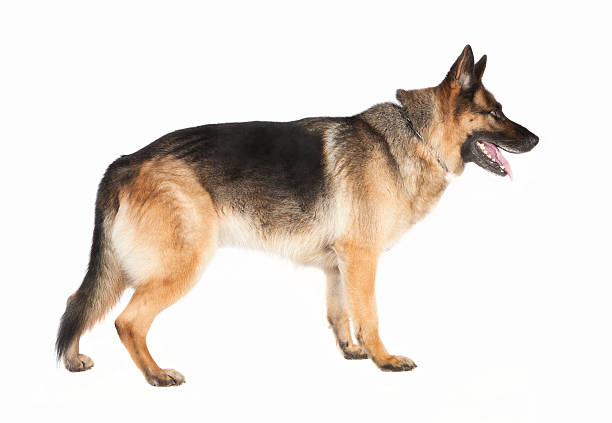
\includegraphics[width=400px]{dog/german sheperd} \caption{Great Dane (XL)}\label{fig:unnamed-chunk-2-3}
\end{figure}

\begin{Shaded}
\begin{Highlighting}[]
\NormalTok{knitr}\SpecialCharTok{::}\FunctionTok{include\_graphics}\NormalTok{(}\StringTok{"dog/Boxer.jpg"}\NormalTok{)}
\end{Highlighting}
\end{Shaded}

\begin{figure}
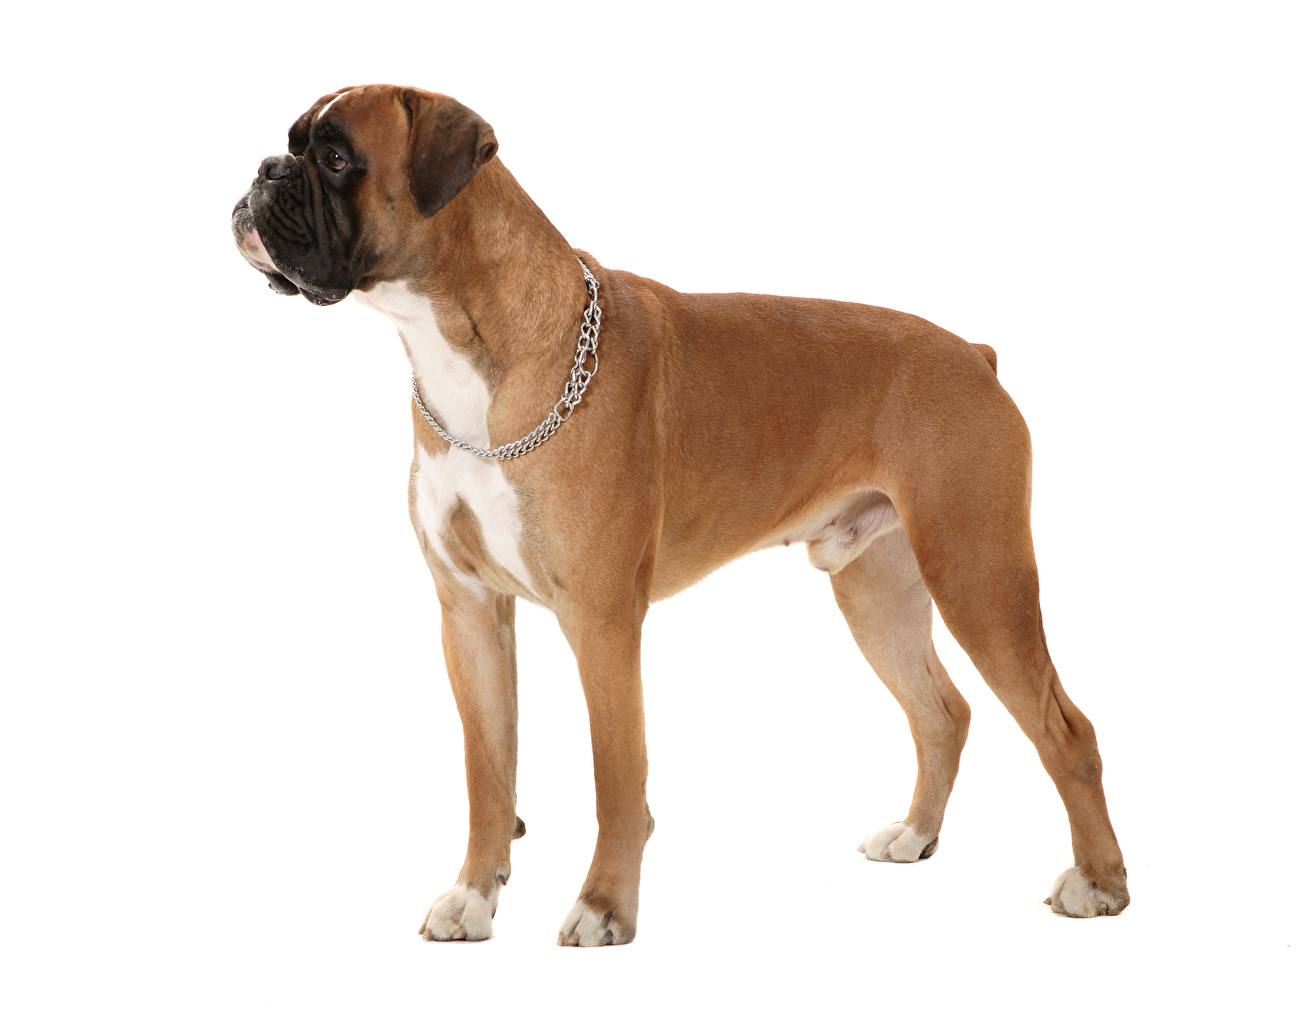
\includegraphics[width=400px]{dog/Boxer} \caption{Golden Retriever (L)}\label{fig:unnamed-chunk-2-4}
\end{figure}

\begin{Shaded}
\begin{Highlighting}[]
\NormalTok{knitr}\SpecialCharTok{::}\FunctionTok{include\_graphics}\NormalTok{(}\StringTok{"dog/greatdane.jpg"}\NormalTok{)}
\end{Highlighting}
\end{Shaded}

\begin{figure}
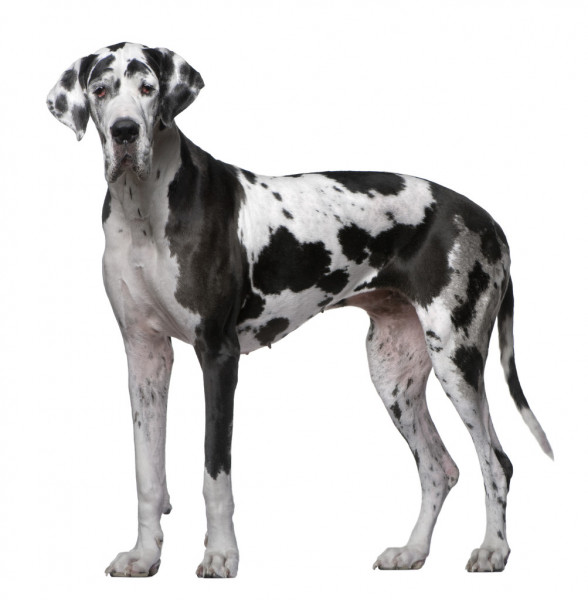
\includegraphics[width=400px]{dog/greatdane} \caption{German Shepherd (L)}\label{fig:unnamed-chunk-2-5}
\end{figure}

\begin{Shaded}
\begin{Highlighting}[]
\CommentTok{\#global variable}
\NormalTok{alignment\_name}\OtherTok{\textless{}\textless{}{-}}\StringTok{""}
\CommentTok{\#notebook functions}

\CommentTok{\#align fasta from file\_name with names from name file (visualization purposes)}
\CommentTok{\#after alignment displays msaprettyprint results for human readable data}
\NormalTok{mult\_alingments}\OtherTok{\textless{}{-}}\ControlFlowTok{function}\NormalTok{(file\_name,fasta\_names,name)\{}
  \CommentTok{\#read in fasta for all dogs}
\NormalTok{  string\_set}\OtherTok{\textless{}{-}}\FunctionTok{readDNAStringSet}\NormalTok{(}\AttributeTok{file=}\NormalTok{file\_name,}\AttributeTok{use.names=}\ConstantTok{FALSE}\NormalTok{)}
  \CommentTok{\#read in seq names as list }
\NormalTok{  table}\OtherTok{=}\FunctionTok{read.table}\NormalTok{(fasta\_names, }\AttributeTok{header =} \ConstantTok{FALSE}\NormalTok{, }\AttributeTok{sep =} \StringTok{"}\SpecialCharTok{\textbackslash{}n}\StringTok{"}\NormalTok{)[[}\StringTok{"V1"}\NormalTok{]]}
  \CommentTok{\#update names for pretty print}
  \FunctionTok{names}\NormalTok{(string\_set)}\OtherTok{\textless{}{-}}\NormalTok{table}
  \CommentTok{\#align unnamed seqs}
\NormalTok{  alignment}\OtherTok{\textless{}{-}}\FunctionTok{msa}\NormalTok{(string\_set)}
  \CommentTok{\#update global variable so multiple pretty print runs dont overrun eachother}
\NormalTok{  alignment\_name}\OtherTok{\textless{}\textless{}{-}}\FunctionTok{gsub}\NormalTok{(}\StringTok{" "}\NormalTok{, }\StringTok{""}\NormalTok{, }\FunctionTok{paste}\NormalTok{(name,}\StringTok{".pdf"}\NormalTok{), }\AttributeTok{fixed =} \ConstantTok{TRUE}\NormalTok{)}
  \CommentTok{\#return pretty alignment, does not show up on my console}
  \FunctionTok{msaPrettyPrint}\NormalTok{(alignment, }\AttributeTok{file=}\NormalTok{alignment\_name,}\AttributeTok{output=}\StringTok{"pdf"}\NormalTok{, }\AttributeTok{showNames=}\StringTok{"right"}\NormalTok{,}\AttributeTok{showLogo=}\StringTok{"top"}\NormalTok{,}\AttributeTok{askForOverwrite=}\ConstantTok{FALSE}\NormalTok{,}\AttributeTok{showNumbering=}\StringTok{"none"}\NormalTok{,}\AttributeTok{paperWidth=}\DecValTok{6}\NormalTok{,}\AttributeTok{paperHeight=}\DecValTok{3}\NormalTok{)}
  \FunctionTok{return}\NormalTok{(alignment\_name)}
\NormalTok{\}}
\CommentTok{\#have figure with white background, no gridline and only axis ticks, no lines}
\NormalTok{tune\_figure}\OtherTok{\textless{}{-}}\ControlFlowTok{function}\NormalTok{(fig,addons)\{}
  \FunctionTok{return}\NormalTok{(fig}\SpecialCharTok{+}\FunctionTok{theme\_minimal}\NormalTok{()}\SpecialCharTok{+}\FunctionTok{theme}\NormalTok{(}
    \AttributeTok{plot.background =} \FunctionTok{element\_blank}\NormalTok{(),}
    \AttributeTok{panel.grid.major =} \FunctionTok{element\_blank}\NormalTok{(),}
    \AttributeTok{panel.grid.minor =} \FunctionTok{element\_blank}\NormalTok{(),}
    \AttributeTok{panel.border =} \FunctionTok{element\_blank}\NormalTok{()))}
\NormalTok{\}}
\CommentTok{\#create dendogram based on fasta files, names of items clustered in fasta\_names, fig\_title is for fig}
\NormalTok{create\_dendogram}\OtherTok{\textless{}{-}}\ControlFlowTok{function}\NormalTok{(fasta\_path, fasta\_names, fig\_title)\{}
\NormalTok{  dna }\OtherTok{\textless{}{-}}\NormalTok{ string\_set}\OtherTok{\textless{}{-}}\FunctionTok{readDNAStringSet}\NormalTok{(}\AttributeTok{file=}\NormalTok{fasta\_path,}\AttributeTok{use.names=}\ConstantTok{FALSE}\NormalTok{)}
  \FunctionTok{names}\NormalTok{(dna)}\OtherTok{=}\FunctionTok{read.table}\NormalTok{(fasta\_names, }\AttributeTok{header =} \ConstantTok{FALSE}\NormalTok{, }\AttributeTok{sep =} \StringTok{"}\SpecialCharTok{\textbackslash{}n}\StringTok{"}\NormalTok{)[[}\StringTok{"V1"}\NormalTok{]]}
\NormalTok{  d1 }\OtherTok{\textless{}{-}} \FunctionTok{DistanceMatrix}\NormalTok{(dna, }\AttributeTok{type=}\StringTok{"dist"}\NormalTok{)}
\NormalTok{  dendogram}\OtherTok{\textless{}{-}}\FunctionTok{IdClusters}\NormalTok{(d1, }\AttributeTok{method=}\StringTok{"complete"}\NormalTok{, }\AttributeTok{cutoff=}\FloatTok{0.05}\NormalTok{, }\AttributeTok{showPlot=}\ConstantTok{FALSE}\NormalTok{,}
                        \AttributeTok{type=}\StringTok{"dendrogram"}\NormalTok{)}
\NormalTok{  nodePar }\OtherTok{\textless{}{-}} \FunctionTok{list}\NormalTok{(}\AttributeTok{lab.cex =} \FloatTok{0.6}\NormalTok{, }\AttributeTok{pch =} \FunctionTok{c}\NormalTok{(}\ConstantTok{NA}\NormalTok{, }\DecValTok{19}\NormalTok{), }
                \AttributeTok{cex =} \FloatTok{0.7}\NormalTok{, }\AttributeTok{col =} \StringTok{"black"}\NormalTok{)}
  \FunctionTok{plot}\NormalTok{(}\FunctionTok{as.dendrogram}\NormalTok{(dendogram), }\AttributeTok{ylab =} \StringTok{"Height"}\NormalTok{, }\AttributeTok{nodePar =}
\NormalTok{         nodePar,}\AttributeTok{main=}\NormalTok{fig\_title)}
\NormalTok{\}}
\end{Highlighting}
\end{Shaded}

LCORL Analysis

\begin{Shaded}
\begin{Highlighting}[]
\CommentTok{\#LCORL CALL}
\NormalTok{alignment}\OtherTok{\textless{}{-}}\FunctionTok{mult\_alingments}\NormalTok{(}\StringTok{"fasta/LCORL\_file.txt"}\NormalTok{,}\StringTok{"fasta/names.txt"}\NormalTok{,}\StringTok{"LCORL"}\NormalTok{)}
\end{Highlighting}
\end{Shaded}

\begin{verbatim}
## use default substitution matrix
\end{verbatim}

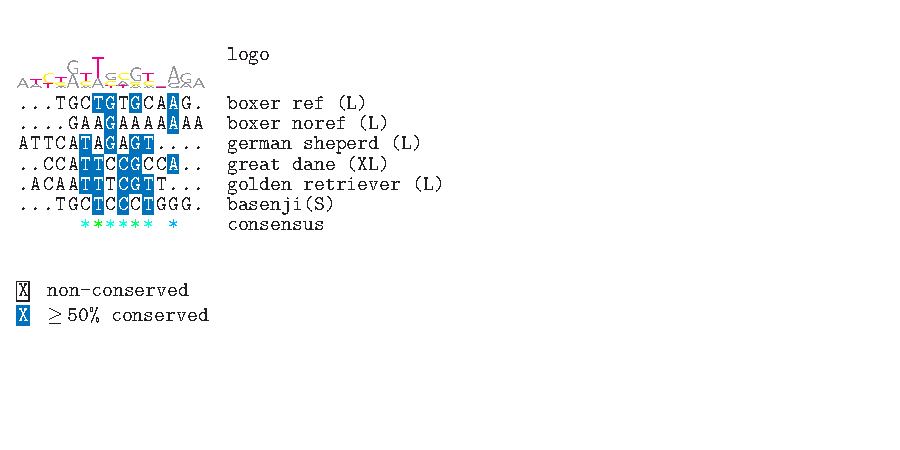
\includegraphics{LCORL.pdf}

\begin{Shaded}
\begin{Highlighting}[]
\CommentTok{\#IGF1 CALL}
\NormalTok{alignment}\OtherTok{\textless{}{-}}\FunctionTok{mult\_alingments}\NormalTok{(}\StringTok{"fasta/igf1.fasta"}\NormalTok{,}\StringTok{"fasta/igf1\_names.txt"}\NormalTok{,}\StringTok{"igf1"}\NormalTok{)}
\end{Highlighting}
\end{Shaded}

\begin{verbatim}
## use default substitution matrix
\end{verbatim}

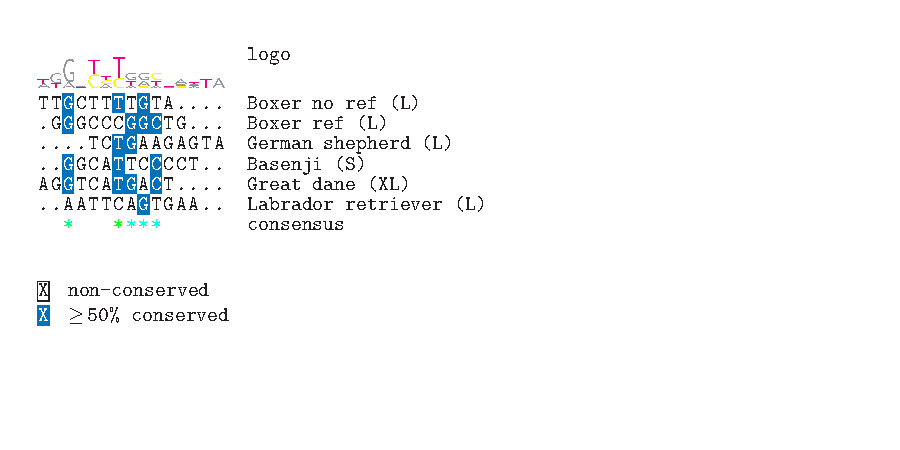
\includegraphics{igf1.pdf}

\begin{Shaded}
\begin{Highlighting}[]
\CommentTok{\#visualize size breakdown of dogs}
\NormalTok{snps}\OtherTok{\textless{}{-}}\FunctionTok{read\_excel}\NormalTok{(}\StringTok{"dog snps.xlsx"}\NormalTok{)}
\CommentTok{\#fix ordering of legend}
\NormalTok{snps}\SpecialCharTok{$}\NormalTok{Name }\OtherTok{\textless{}{-}} \FunctionTok{factor}\NormalTok{(snps}\SpecialCharTok{$}\NormalTok{Name, }\AttributeTok{levels =} \FunctionTok{c}\NormalTok{(}\StringTok{"Basenji"}\NormalTok{, }\StringTok{"Boxer"}\NormalTok{, }\StringTok{"German\_Shepherd"}\NormalTok{,}\StringTok{"Labrador\_retriever"}\NormalTok{,}\StringTok{"Great\_Dane"}\NormalTok{))}
\NormalTok{p}\OtherTok{\textless{}{-}}\FunctionTok{ggplot}\NormalTok{(}\AttributeTok{data =}\NormalTok{ snps, }\FunctionTok{aes}\NormalTok{(size))}\SpecialCharTok{+}\FunctionTok{scale\_x\_discrete}\NormalTok{(}\AttributeTok{limits =} \FunctionTok{c}\NormalTok{(}\StringTok{"S"}\NormalTok{,}\StringTok{"L"}\NormalTok{,}\StringTok{"XL"}\NormalTok{))}\SpecialCharTok{+}\FunctionTok{geom\_bar}\NormalTok{(}\FunctionTok{aes}\NormalTok{(}\AttributeTok{fill =}\NormalTok{ Name))}\SpecialCharTok{+}\FunctionTok{scale\_fill\_manual}\NormalTok{(}\AttributeTok{values =} \FunctionTok{c}\NormalTok{(}\StringTok{"deepskyblue4"}\NormalTok{,}\StringTok{"brown2"}\NormalTok{,}\StringTok{"brown"}\NormalTok{,}\StringTok{"brown4"}\NormalTok{,}\StringTok{"darkseagreen4"}\NormalTok{))}
\FunctionTok{tune\_figure}\NormalTok{(p,add\_ons)}
\end{Highlighting}
\end{Shaded}

\includegraphics{Untitled_files/figure-latex/unnamed-chunk-8-1.pdf}

\begin{Shaded}
\begin{Highlighting}[]
\CommentTok{\#visualize IGF1 SNP by size }
\NormalTok{p}\OtherTok{\textless{}{-}}\FunctionTok{ggplot}\NormalTok{(}\AttributeTok{data =}\NormalTok{ snps, }\AttributeTok{mapping =} \FunctionTok{aes}\NormalTok{(}\AttributeTok{y=}\NormalTok{igf1,}\AttributeTok{x=}\NormalTok{size\_num))}\SpecialCharTok{+}\FunctionTok{geom\_point}\NormalTok{(}\AttributeTok{size=}\DecValTok{4}\NormalTok{,}\AttributeTok{alpha=}\FloatTok{0.6}\NormalTok{,}\AttributeTok{color=}\StringTok{"darkseagreen4"}\NormalTok{)}
\NormalTok{p}\SpecialCharTok{+}\FunctionTok{geom\_jitter}\NormalTok{(}\AttributeTok{size=}\DecValTok{4}\NormalTok{,}\AttributeTok{alpha=}\FloatTok{0.6}\NormalTok{,}\AttributeTok{color=}\StringTok{"darkseagreen4"}\NormalTok{)}
\end{Highlighting}
\end{Shaded}

\includegraphics{Untitled_files/figure-latex/unnamed-chunk-9-1.pdf}

\begin{Shaded}
\begin{Highlighting}[]
\CommentTok{\#visualize LCORL SNP by size }
\NormalTok{p}\OtherTok{\textless{}{-}}\FunctionTok{ggplot}\NormalTok{(}\AttributeTok{data =}\NormalTok{ snps, }\AttributeTok{mapping =} \FunctionTok{aes}\NormalTok{(}\AttributeTok{y=}\NormalTok{lcorl,}\AttributeTok{x=}\NormalTok{size\_num))}\SpecialCharTok{+}\FunctionTok{geom\_point}\NormalTok{(}\AttributeTok{size=}\DecValTok{4}\NormalTok{,}\AttributeTok{alpha=}\FloatTok{0.6}\NormalTok{,}\AttributeTok{color=}\StringTok{"darkseagreen4"}\NormalTok{)}
\NormalTok{p}\SpecialCharTok{+}\FunctionTok{geom\_jitter}\NormalTok{(}\AttributeTok{size=}\DecValTok{4}\NormalTok{,}\AttributeTok{alpha=}\FloatTok{0.6}\NormalTok{,}\AttributeTok{color=}\StringTok{"darkseagreen4"}\NormalTok{)}
\end{Highlighting}
\end{Shaded}

\includegraphics{Untitled_files/figure-latex/unnamed-chunk-10-1.pdf}

\begin{Shaded}
\begin{Highlighting}[]
\CommentTok{\#Cluster LCORL extended fragment }
\FunctionTok{create\_dendogram}\NormalTok{(}\StringTok{"fasta/LCORL\_file.txt"}\NormalTok{, }\StringTok{"fasta/names.txt"}\NormalTok{, }\StringTok{"LCORL Extended Fragment Dendogram"}\NormalTok{)}
\end{Highlighting}
\end{Shaded}

\begin{verbatim}
## ================================================================================
## 
## Time difference of 0 secs
## 
## ================================================================================
## 
## Time difference of 0.01 secs
\end{verbatim}

\includegraphics{Untitled_files/figure-latex/unnamed-chunk-11-1.pdf}
\url{http://www.sthda.com/english/wiki/beautiful-dendrogram-visualizations-in-r-5-must-known-methods-unsupervised-machine-learning\#plot.dendrogram-function}
for look and non cut off stuff

\begin{Shaded}
\begin{Highlighting}[]
\CommentTok{\#Cluster IGF1 extended fragment }
\FunctionTok{create\_dendogram}\NormalTok{(}\StringTok{"fasta/igf1.fasta"}\NormalTok{, }\StringTok{"fasta/igf1\_names.txt"}\NormalTok{, }\StringTok{"IGF1 Extended Fragment Dendogram"}\NormalTok{)}
\end{Highlighting}
\end{Shaded}

\begin{verbatim}
## ================================================================================
## 
## Time difference of 0 secs
## 
## ================================================================================
## 
## Time difference of 0.01 secs
\end{verbatim}

\includegraphics{Untitled_files/figure-latex/unnamed-chunk-12-1.pdf}

\end{document}
